%! TEX root = analisis_bising_temu9.tex
% the main TeX file which is intended to compile, :VimtexReload after adjustment
% :h vimtex-tex-root
\documentclass[../main.tex]{subfiles}
% \includeonlyframes{current}
% \setbeameroption{hide notes} % Only slides
% \setbeameroption{show only notes} % Only notes
% \setbeameroption{show notes on second screen=right} % Both

\begin{document}
\begin{frame}[mytitle=standard,c,mycolor=digiPH_cream,light]
	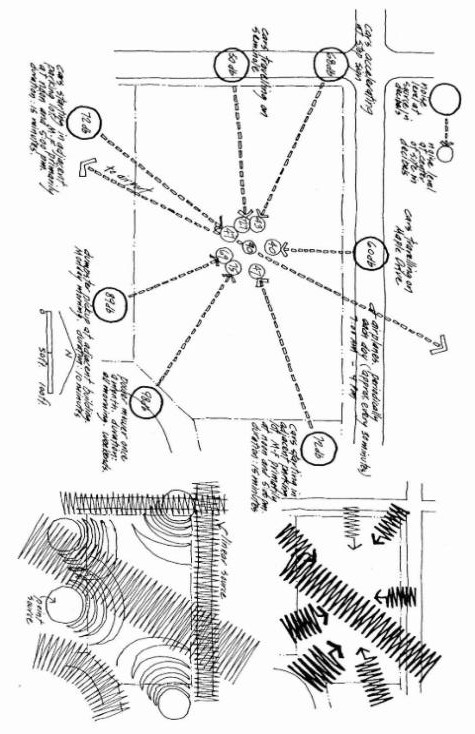
\includegraphics[width=.7\textwidth, angle=90]{../figures/bising.jpg}
\end{frame}
\bgdarkimg{bising_2}
\bgdarkimg{bising_cth}
\bgdarkimg{akses_lingkungan_bising_cth}
\bgdarkimg{semua_cth}
\bgdarkimg{iklim_2_cth}

\end{document}
